\chapter{集成测试与持续集成测试}
\label{cha:intro}

本章首先对集成测试的理论和发展进行了概述,最后介绍了当前处于快速发展时期的敏捷开发所对应的持续集成测试,为后续UEFI BIOS自动化测试系统的设计与实现铺垫好了理论。

\section{集成测试}

\subsection{集成测试的概念}

  集成测试是一种旨在暴露模块单元接口之间、组件和系统间交互或者协同工作时所存在的缺陷的测试,重在接口的测试。它通过一定的方法,将已研发并且单独测试好的模块或者单元,通过设计好的产品规则集成为所需要的产品,并且测试该产品以保证产品能够正常的工作并且符合设计的目的,这一过程被称为集成测试。在进行集成时要注意下列几个注意点:
  
  \begin{itemize}
    \item 在将每个已经测试好的组成模块集成起来之后,经过模块输入输出接口的数据是不是会丢失。
	\item 某个正常执行的模块是不是会影响其他模块的正常工作。
	\item 每个各自正常工作功能的模块按照一定的需求和规则一起组合运行时,是不是能够完成设计所期待的效果。
	\item 全局的数据结构是否存在缺陷。
	\item 每一个模块可能都会存在误差,当他们积累到一起的时候,与期待结果的相差值会不会被放大,并且超过了设计时所不能接受的范围。
  \end{itemize}
  
  不同情况下不同层次的集成测试主要分为:

  \begin{itemize}
    \item 软件单元与软件单元的集成测试。
	\item 软件每个系统之间的集成测试。
	\item 软件系统和第三方系统的集成测试。
	\item 软件系统和硬件的集成测试。
  \end{itemize}
  
\subsection{软件开发模型与集成方法的对比研究}

  从集成方式看,瀑布模型对应的大棒集成、统一软件开发过程对应的渐增式集成以及敏捷软件开发中的持续集成,是最具有里程碑意义的三个阶段。如图~\ref{fig:从Big-Bang到持续集成的发展过程}所示:

  	\begin{figure}[H] % use float package if you want it here
		\centering
		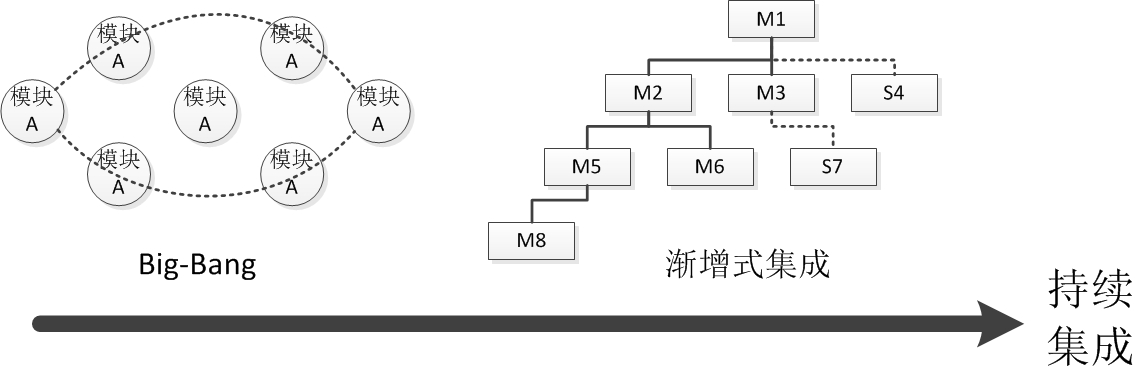
\includegraphics[height=4.8cm]{chart2/从Big-Bang到持续集成的发展过程}
		\caption{从Big-Bang到持续集成的发展过程}
		\label{fig:从Big-Bang到持续集成的发展过程}
	\end{figure}
  
  \begin{itemize}
	\item 瀑布模型与大棒集成模式
	
	Winston Royce~\cite{34}提出了瀑布模型~\cite{35},它认为软件产品研发的阶段应该分为五个,如图~\ref{fig:瀑布模型}所示:
	
	\begin{figure}[H] % use float package if you want it here
		\centering
		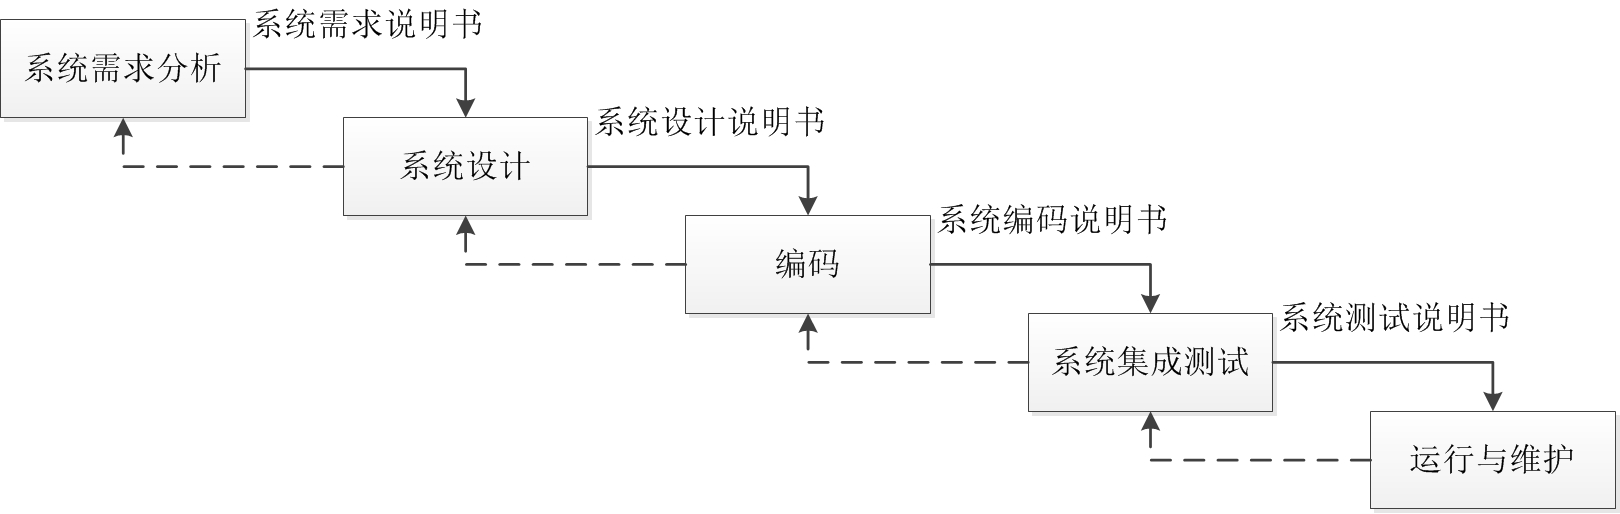
\includegraphics[height=4.5cm]{chart2/瀑布模型}
		\caption{瀑布模型}
		\label{fig:瀑布模型}
	\end{figure}
	
	当系统集成测试时各模块首次被结合起来之后,会有许多之前没有的问题涌现出来,其中一个模块出现问题之后,需要调试系统所有的部分才能定位缺陷的位置。通常把这种集成方式称之为大棒集成~\cite{36}。
	
	\item 统一软件开发过程与渐增式集成模式
			
	软件统一开发过程~\cite{37}认为,项目的开发应该通过数次迭代将其划分为若干个小的阶段,每一个迭代周期都应该包含各自对应的产品需求分析、系统设计、产品编码和软件测试等过程,每个周期结束后,应该对其结果按照各阶段的标准进行评判,若达到标准则制定下一周期的目标并且进入一轮新的迭代。如图~\ref{fig:迭代递增过程模型}所示:

	\begin{figure}[H] % use float package if you want it here
		\centering
		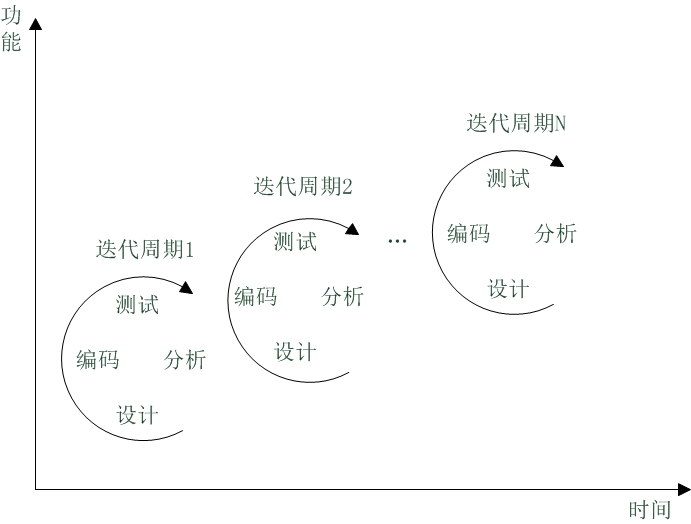
\includegraphics[height=7.5cm]{chart2/迭代递增过程模型}
		\caption{统一软件开发过程模型}
		\label{fig:迭代递增过程模型}
	\end{figure}
	
	\item 敏捷软件开发与持续集成
	
	敏捷开发方法~\cite{41}(Agile Methodologies,以下简称敏捷方法)针对现代商业软件业务复杂、需求频繁变化、开发周期短等问题,其通过以下几点来在整个软件开发的进程中大大缩减项目的成本:

	  \begin{itemize}
		\item 在产品开发开始后的第一到第三周尽快发布第一个版本,以便于能够尽快的得到反馈,并且在其基础上进一步开发。		
		\item 解决方案尽量不要太复杂,以便于在之后对其进行修改。
		\item 不断改进设计,提高设计的质量。
		\item 在每一个迭代的周期一直对产品测试和验证,从而在开发后期降低产品测试和缺陷改正的成本。
	  \end{itemize}
	
	敏捷软件开发方法认为,在对产品源文件做出一定修改后,就应当尽快集成和测试整个产品,反馈得到其结果,以验证之前的操作是否合理,这便是持续集成。
	
  \end{itemize}
  
  
\section{持续集成测试}

\subsection{持续集成的概念}

	作为持续集成的指导思想,软件开发者们认为,应该频繁的对整个软件产品项目的源代码库进行集成,甚至于任何一个对其的修改动作在提交到项目所对应的版本控制库之后,系统都应该触发一次针对该版本的集成工作,这对于整个软件项目工程的好处是非常大的,有助于产品缺陷及时暴露。而敏捷思想的重要体现之一,正是如何将软件的集成工作变为自动化的持续以及寻找最合适的极致点。~\cite{13}
	
	2006年,Martin Fowler阐述并且实现了持续集成这一重要思想:
	
	\begin{itemize}
		\item 软件产品项目的工程通常有大量的源文件,在产品的编译构建过程中需要包含数量庞大的文件,为了方便管理整个项目,应该创建单个产品的源码库,利用其保留所有这些文件的修改记录,并且这些修改记录是可以被追溯历史的,这一点非常重要。
		\item 在软件项目开发的过程中,开发者们会对产品的源代码进行频繁的重构和修改,在每次修改动作完成时,其都应该将本地修改的代码与源码库中的主干进行合并,频率上至少应该保证每天提交一次。这样有助于其他的软件开发人员清晰的了解源文件的变更情况,而少量的、及时的将修改提交到源码库,可以尽早的验证该操作的正确性,从而避免在产品后期集成时产品缺陷的集中涌现,大大减少代码回滚的成本以及修复产品缺陷的成本。
		\item 为了将产品的源码编译构建成为可正确执行的程序,软件开发人员通常需要从源码库中获取相应版本的产品源文件,并且利用相应的工具对产品的源码进行构建,将这些机械固定的操作利用相关的技术自动化的完成,有助于减少他们的时间成本,因此产品的构建过程需要能够自动化的完成。
		\item 为了保证开发人员对代码的每次修改操作的正确性,应该将其对应版本源码库中的源码进行集成构建。若构建失败则该操作错误,需要退回到修改之前的版本并且重新进行修改;若构建成功,则需要对产品进行环境部署并且加以相应的测试,已验证产品的正确性,如果存在产品的缺陷则应该及时的修复。
		\item 编译构建成功后的产品,应该部署到其相应的真实环境中去,并且利用相关的技术对产品进行测试,而这一系列的操作需要能够自动化的完成,而不需要人为机械的去手动操作。测试完成后,为了方便软件开发人员清晰的了解到最新版本产品的集成和测试结果,判断其对应的开发操作是否正确,持续集成系统应该能够自动的生成其对应的测试报告,并且将其按时反馈给每一个开发人员。
	\end{itemize}
	
	\begin{figure}[H] % use float package if you want it here
		\centering
		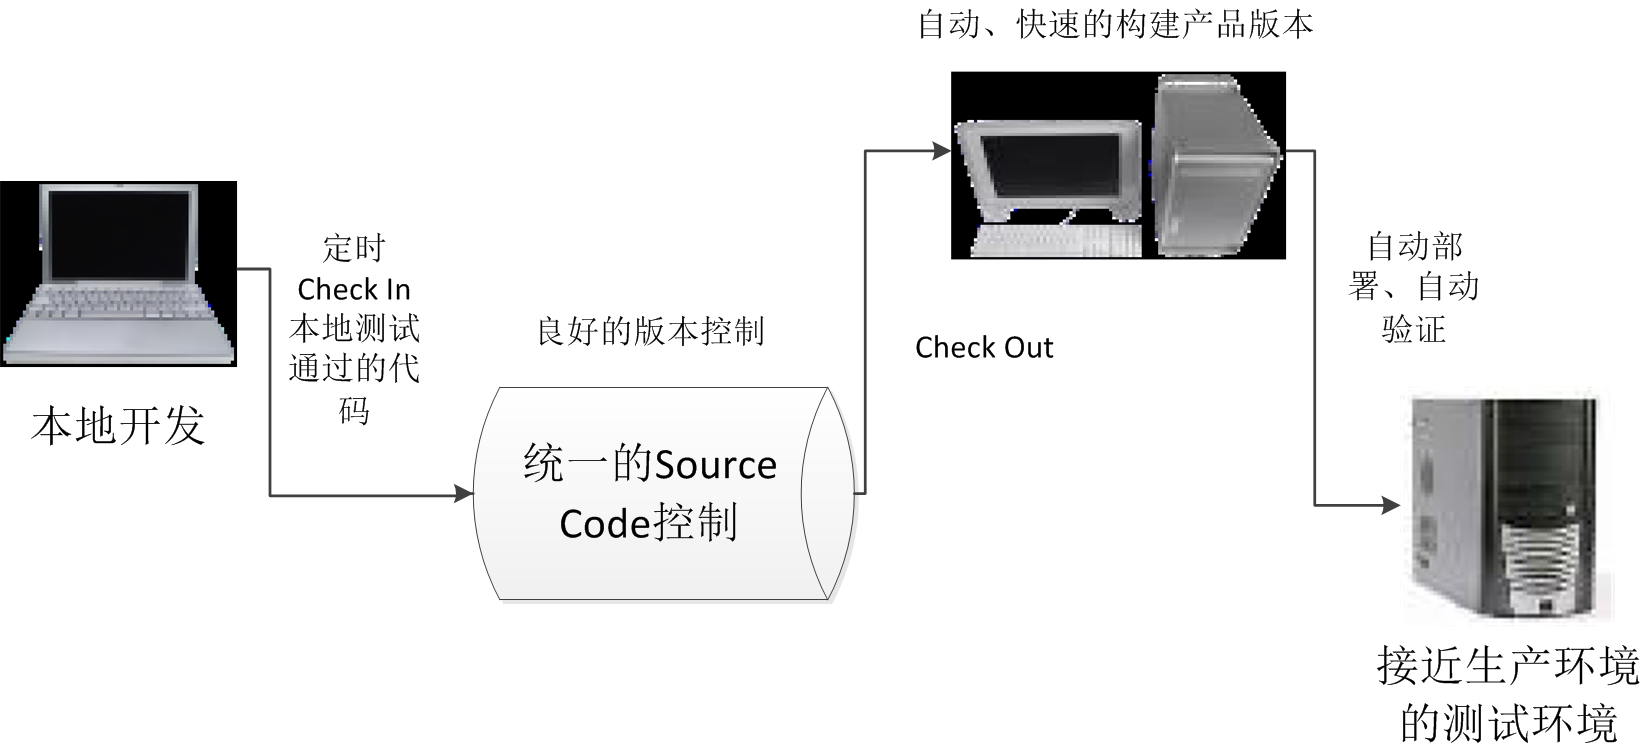
\includegraphics[height=6.5cm]{chart2/简化版持续集成}
		\caption{简化版持续集成}
		\label{fig:简化版持续集成}
	\end{figure}
	
\subsection{持续集成的价值}

	\begin{itemize}
		\item 系统中的任一环节都是自动完成的,有利于减少测试任务中的重复过程所耗费的时间和人力成本。
		\item 系统能够尽早、及时的发现软件不能够构建或者存在产品缺陷的问题,使随时(快速、可靠、低风险)发布功能正常的软件成为了可能。
		\item 系统尽早、尽快进行集成,有助于尽早发现产品中存在的缺陷,避免最终产品集成中出现Bug大量涌现的情况,这样容易及时定位和修正Bug,提高产品开发的质量与效率。
		\item 保证了敏捷开发过程中软件项目的进度和产品的质量。
	\end{itemize}
	
	\begin{figure}[H] % use float package if you want it here
		\centering
		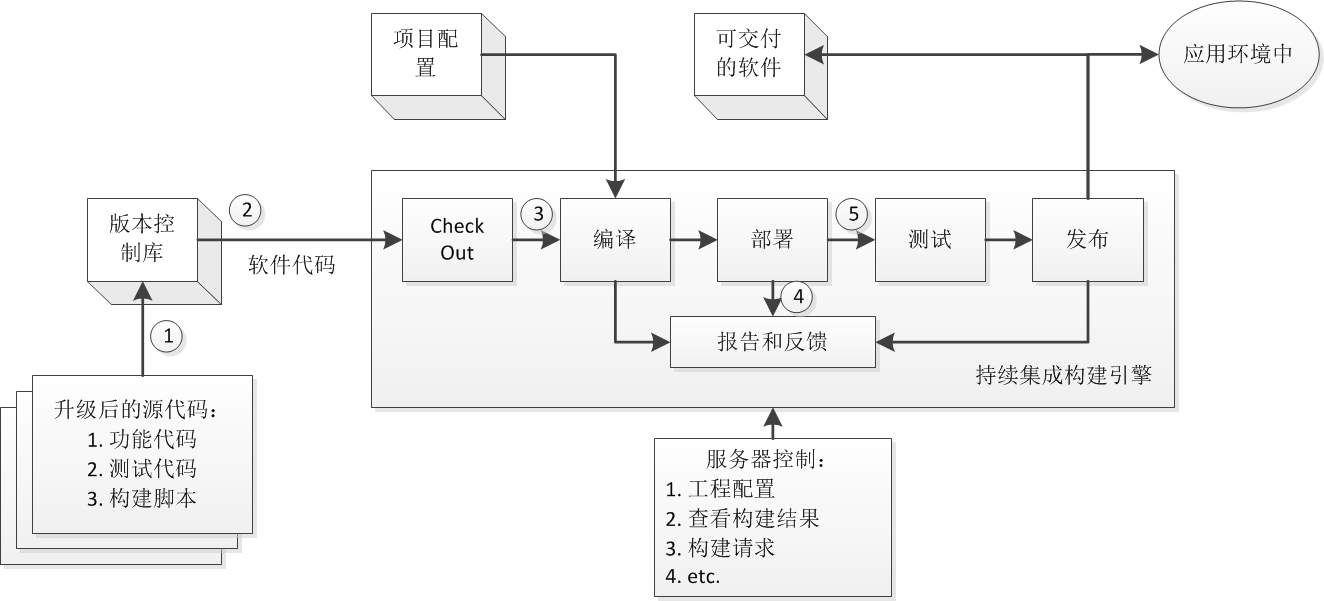
\includegraphics[height=7cm]{chart2/典型的持续集成开发场景}
		\caption{典型的持续集成开发场景}
		\label{fig:典型的持续集成开发场景}
	\end{figure}
	
\section{持续集成的组成}

	为了针对产品的特点,设计和开发的持续集成测试系统,其中所用到的每一个模块,以及其所组成的系统,都需要利用相应的自动化技术以及相应的工具。按照系统的需求,选择合适的技术与工具,寻求相应的方法与规则将它们结合到一起加以利用,才能够根据产品和测试操作的需求目的,实现其对应的系统,完成自动化的持续集成操作。这些工具和自动化技术如图~\ref{fig:与持续集成应用相关的软件工具和自动化技术}所示:
	
	\begin{figure}[H] % use float package if you want it here
		\centering
		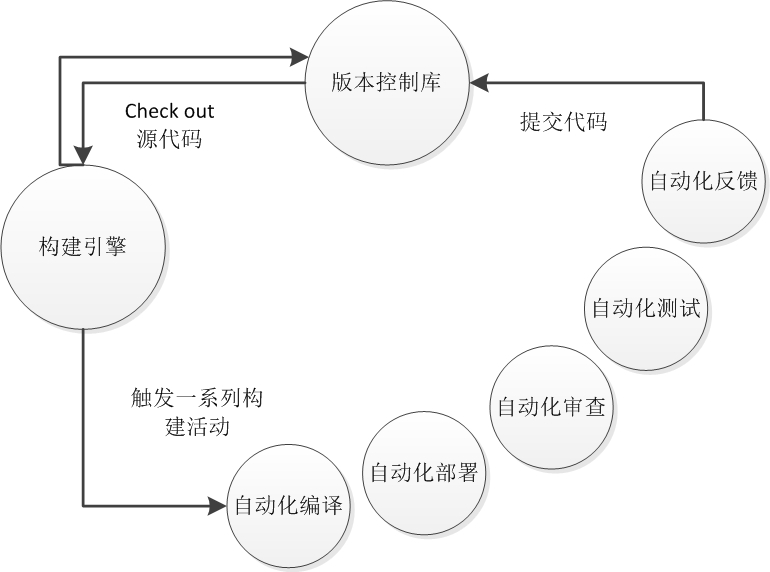
\includegraphics[height=7cm]{chart2/与持续集成应用相关的软件工具和自动化技术}
		\caption{与持续集成应用相关的软件工具和自动化技术}
		\label{fig:与持续集成应用相关的软件工具和自动化技术}
	\end{figure}
	
	这些自动化技术和相应的工具主要由产品的自动化构建技术、版本控制库、持续集成的构建引擎、版本控制系统所创建的版本控制库所组成。其中自动化构建与测试操作是CI持续集成测试系统的核心部分,由自动化编译构建、自动化产品测试、自动化审查、自动化环境部署、自动化报告反馈等技术组成。
	
	\subsection{持续集成的环境}
	
	持续集成的环境主要由图~\ref{fig:持续集成环境基本框架的体系结构图}中的各要素组成:
	
	\begin{figure}[H] % use float package if you want it here
		\centering
		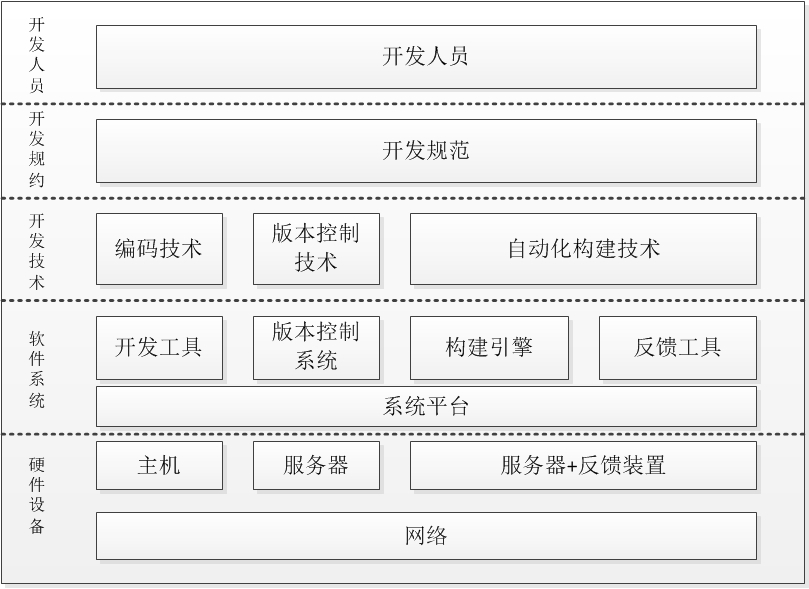
\includegraphics[height=8cm]{chart2/持续集成环境基本框架的体系结构图}
		\caption{CI环境基本框架的体系结构图}
		\label{fig:持续集成环境基本框架的体系结构图}
	\end{figure}
	
	\subsection{版本控制}

	软件产品工程的项目通常需要利用一个能够存放源代码的仓库来管理其对应的源文件,通常利用现有的版本控制系统来创建其对应的源代码仓库,利用其管理整个项目的源文件。版本控制系统能够进行有效的管理产品的源代码,开发人员在修改源码并对其提交后,版本控制系统都能够对其操作进行记录,并且在源码的修改出现问题时,利用其代码的可追溯性,根据代码的提交时间点,把源代码恢复到某个之前的版本。除此之外,利用其使得不同国家和地区的人们可以通过网络实现产品的协同开发。
	
	版本控制系统大致分为以下两种:
	
	\begin{itemize}
		\item 集中式版本控制系统
		
			集中式版本控制系统的原理,是利用一台服务器来保存所有修改版本的源文件,项目中共同协作的软件开发人员通过自己的客户端连接到这台服务器,服务器对其进行集中式的管理操作,开发人员可以利用各自的客户端从服务器中获取最新版本的源文件,并且能够将在本地修改的源文件作为新的版本提交更新到服务器中,为他人所获取。现如今常用的集中式版本控制系统主要有Subversion(SVN)、Concurrent Versions System(CVS)以及 Perforce 等。
			
			\begin{figure}[H] % use float package if you want it here
				\centering
				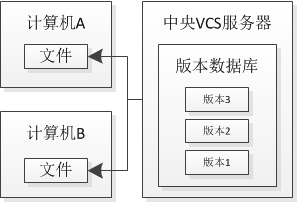
\includegraphics[height=5cm]{chart2/集中式版本控制系统}
				\caption{集中式版本控制系统}
				\label{fig:集中式版本控制系统}
			\end{figure}
		\item 分布式版本控制系统
		
			而在分布式版本控制系统中,每一个开发人员的计算机并不仅仅只是客户端,用于向版本控制库提交或者从版本控制库中提取最新一个版本的源文件,而且作为服务器把整个仓库全部作为镜像备份,每个成员可用于从中进行获取。开发人员对其的每一次克隆操作,事实上也都是完整备份所有版本的源代码仓库,所以当任何一处服务器发生故障无法正常运行时,其他的每一台服务器都有各自的一个镜像,并且可以利用对本地仓库来进行恢复。目前常用的集中式版本控制系统有Git、Mercurial、Bazaar 以及 Darcs 等,其中以Git最具有代表性和广泛使用性。
			
			\begin{figure}[H] % use float package if you want it here
				\centering
				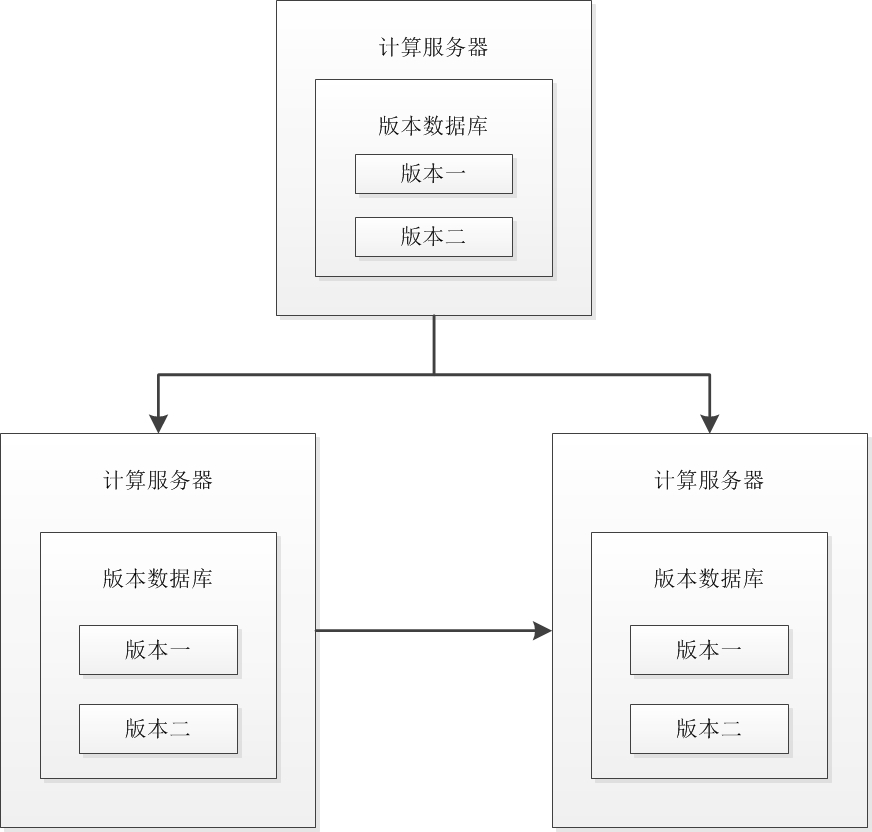
\includegraphics[height=9.5cm]{chart2/分布式版本控制系统}
				\caption{分布式版本控制系统}
				\label{fig:分布式版本控制系统}
			\end{figure}
	\end{itemize}

	\subsection{产品构建}
	
	产品构建环节,是指通过自动化编译技术将产品的源文件编译构建为可最终正常运行的可执行程序的过程。通常情况下利用现有成熟的自编译工具,即可完成产品的编译和构建,例如针对C、C++语言的Unix和Linux下的make工具、Java开发中的Jinx、Maven和Ant工具~\cite{43, 44, 45},以及.NET下的MSBuild工具。
	
	\subsection{环境部署}
	
	在产品构建完成之后系统对环境进行部署,执行如下流程:将已编译构建好的所需验证的可执行文件安装放置其相应的环境中,以便于后续对其进行相应的功能或者性能测试。实现自动化的环境部署的意义是令乏味、机械、重复的环境部署工作不需要人工去操作,从而大大节省了测试人员的成本。	
	
	\subsection{产品测试}
	
	产品测试是CI中最为关键的组成部分,用于检测出产品中存在的缺陷。CI的产品测试工作主要以单元测试~\cite{46}和功能测试为主,性能测试为辅。比较有代表性单元测试工具有:针对.NET 的nUnit、针对Python的pyUnit、针对C++的CppUnit、针对Delphi的dUnit等工具。利用这些现有的工具和技术,能够大大简化开发人员在不同平台和语言上的测试操作,节省他们的成本,提高测试的效率。
	
	\subsection{报告反馈}
	
	产品测试结束后,应该能够自动的解析测试结果生成测试报告,并且将产品的构建结果与测试结果以报告的形式通过电子邮件(Email)、Socket、FTP、HTTP、聚合内容(RSS)等形式途径,及时快速的反馈到所有项目相关的软件开发与测试人员手中,这就是测试反馈部分所需要做的工作内容。
	
\section{现有的持续集成引擎的分析与对比}
	
	为了实现持续集成的自动化,需要使用合适的技术和途径,及时发现版本控制库中源文件的修改与变更情况,若出现变更,应及时自动化的触发集成测试任务,自动化的完成从产品构建、环境部署以及产品测试的过程,并且利用自动化测试反馈的技术,解析测试结果自动生成相应的测试报告,并通过2.3.6小结所提到的形式及时迅速的将结果反馈给开发人员。而这一过程的控制主要由持续集成引擎完成,它是使集成测试做到持续的关键所在。
	
	\subsection{现有的持续集成引擎}
	
	目前专用于持续集成的引擎越来越多,其中常用到的产品有:Cruisecontrol~\cite{47}、Jenkins、QuickBuild和Anthill~\cite{48}等。以下简单介绍两款常用的产品:

	\begin{itemize}
		\item CruiseControl
		
		CruiseControl是最早出现的持续集成引擎之一,由Build Loop作为主体和部分插件所构成。其主体使用轮询机制来定时检测产品源代码的版本,当发现版本更改之后,其可以读取config.xml配置文件中的配置信息,利用其作为准则,调用例如:Ant、Maven等相应的构建工具,以对产品进行自动化的构建。利用RSS、IM、Email 等反馈策略,CruiseControl能够将产品构建的结果尽早、及时的反馈给项目组中相关的成员,以保证最新版本的源代码的有效性。
		\item Jenkins
		
		作为开源软件的代表作之一,Jenkins这款持续集成引擎工具,近些年来在市场中的占有率在不断提升,其广泛应用的程度可想而知。Jenkins具备支持插件、简单的配置安装、监控的可视化这一些特点功能,不仅如此,其具有较快的版本更新能力,通常会每周一次进行版本更新,此外不得不提的是其在GitHub上具备较强的主导能力。这一系列的特点使得这款工具成为了持续集成引擎的代表作,并且在持续集成这一领域的占有率遥遥领先。~\cite{26, 27}
	\end{itemize}
	
	\subsection{现有持续集成引擎的对比}
	
	现有几款常用的持续集成引擎的对比如表~\ref{tab:现有几款主流持续集成引擎的对比}所示:
	
	\begin{table}[H]
		\centering
		\caption{现有几款主流持续集成引擎的对比}
		\label{tab:现有几款主流持续集成引擎的对比}
		\begin{center}
		\begin{tabular}{|p{2.4cm}|p{3.8cm}|p{3.8cm}|p{3.8cm}|} 
		\hline
		{\diagbox[width=2.8cm]{属性}{种类}} & Jenkins & QuickBuild & CruiseControl \\ \hline
		运行的操作系统环境 & 所有的操作系统平台 & Windows 、Linux、Solaris等操作系统平台 & Windows、Unix、Linux以及任何能够正常运行Java虚拟机的操作系统平台 \\ \hline
		特点 & 目前应用最广的集成服务器,具备强大的可扩展插件的特点,开源 & 大型公司对其较多使用,可跨多种平台 & 较适合.NET 开发与Java开发,可跨平台使用 \\ \hline
		可扩展性 & 具备较强的可扩展性,插件库中的内容丰富,可选择程度较高 & 商业软件,不可扩展 & 可扩展,有较多现有的插件供使用 \\ \hline
		版本控制系统的可支持性 & 支持Subversion、CVS、ClearCase、Git等所有主流的集中式与非集中式版本控制系统 & 常用的版本控制系统均可支持使用,较新的版本对GitHub进行了集成 & Subversion、CVS、ClearCase等集中式版本控制系统 \\ \hline
		更新频率 & 更新频率极高 & 更新频率较高 & 版本较旧,更新频率较低 \\ \hline
		易用性 & 极为易用,便于快速部署搭建,维护起来较为简单,具备多种启动方式 & 较为易用,且可用其对大集群服务器进行部署,稳定 & 较难使用,部署和维护的成本高,配置文件过多不利于使用 \\ \hline
		\end{tabular}
		\end{center}
	\end{table}
	
\section{现有持续集成与UEFI BIOS持续集成的分析与对比}
	
	UEFI BIOS产品的开发是一个长期的项目,项目的开发采用敏捷开发的方式,在开发过程中,每一个短暂的迭代周期都会对代码进行频繁的重构和修改,每一次修改都会产生一个新版本的可执行产品,因此QA需要尽早对产品进行集成和测试,这样可以大大避免在项目后期产品进行集成时出现产品缺陷集中涌现的问题。然而随着项目开发过程的进行,QA的测试工作任务量会不断的提升和累加,如果采用手动测试机械重复的完成这些繁重的测试任务,毫无疑问是不明智也是低效的,因此为了节省测试工作的时间和人力成本、提高测试工作的执行效率、保障测试工作的顺利进行和高质量进行,搭建一个自动化持续集成测试系统用于完成从产品构建、产品部署、产品测试以及产品质量分析的UEFI BIOS集成测试工作就显得非常必要。
	
	由于现有的持续集成的各个阶段均是工作在OS(Operation System,操作系统)中的,而UEFI BIOS是工作在OS(Operation System)之下,其源代码的管理、产品的构建虽然是在OS中完成的,但是其环境的部署、产品的测试需要涉及到在非OS的情况下完成,因此现有的各种CI引擎、环境部署和自动化测试工具并不能够实际的应用到UEFI BIOS的测试工作中,需要寻求新的解决方法,甚至开发新的工具,并且利用合适的技术将持续集成的各个阶段在OS与非OS的情况整合到一起,来完成该套UEFI BIOS持续集成测试系统的开发。
	
	针对不同CPU架构以及不同的计算机硬件环境,UEFI BIOS的分类有很多种。在本论文中,我们以Denlow和Nt32两种平台为例,来说明在这两种平台下的自动化测试系统框架的搭建。最终的完成目标是:在IA-32架构(特定的CPU架构)的Nt32平台和X-64架构(特定的CPU架构)的Denlow平台上,实现对该两种不同架构的不同平台的UEFI BIOS持续集成测试系统的搭建。
	
\section{本章小结}
    本章首先对集成测试理论的发展进行了概述,最后介绍了当前处于快速发展时期的敏捷开发所对应的持续集成测试,为后续UEFI BIOS自动化持续集成测试系统的搭建奠定了理论基础。
	
	2.5小结主要将现有持续集成技术与UEFI BIOS持续集成的需求进行了对比。